\documentclass[tikz, border=10pt]{standalone}
\usepackage{tikz}
\usepackage{amsmath, amssymb}
\usetikzlibrary{arrows.meta, positioning, calc}

\definecolor{cGreen}{RGB}{167,210,167}
\definecolor{cPurple}{RGB}{196,175,222}
\definecolor{cBlue}{RGB}{159,197,232}
\definecolor{cGray}{RGB}{215,215,215}
\definecolor{cYellow}{RGB}{255,229,153}
\definecolor{cOrange}{RGB}{255,193,120}
\definecolor{cRed}{RGB}{234,153,153}

\begin{document}
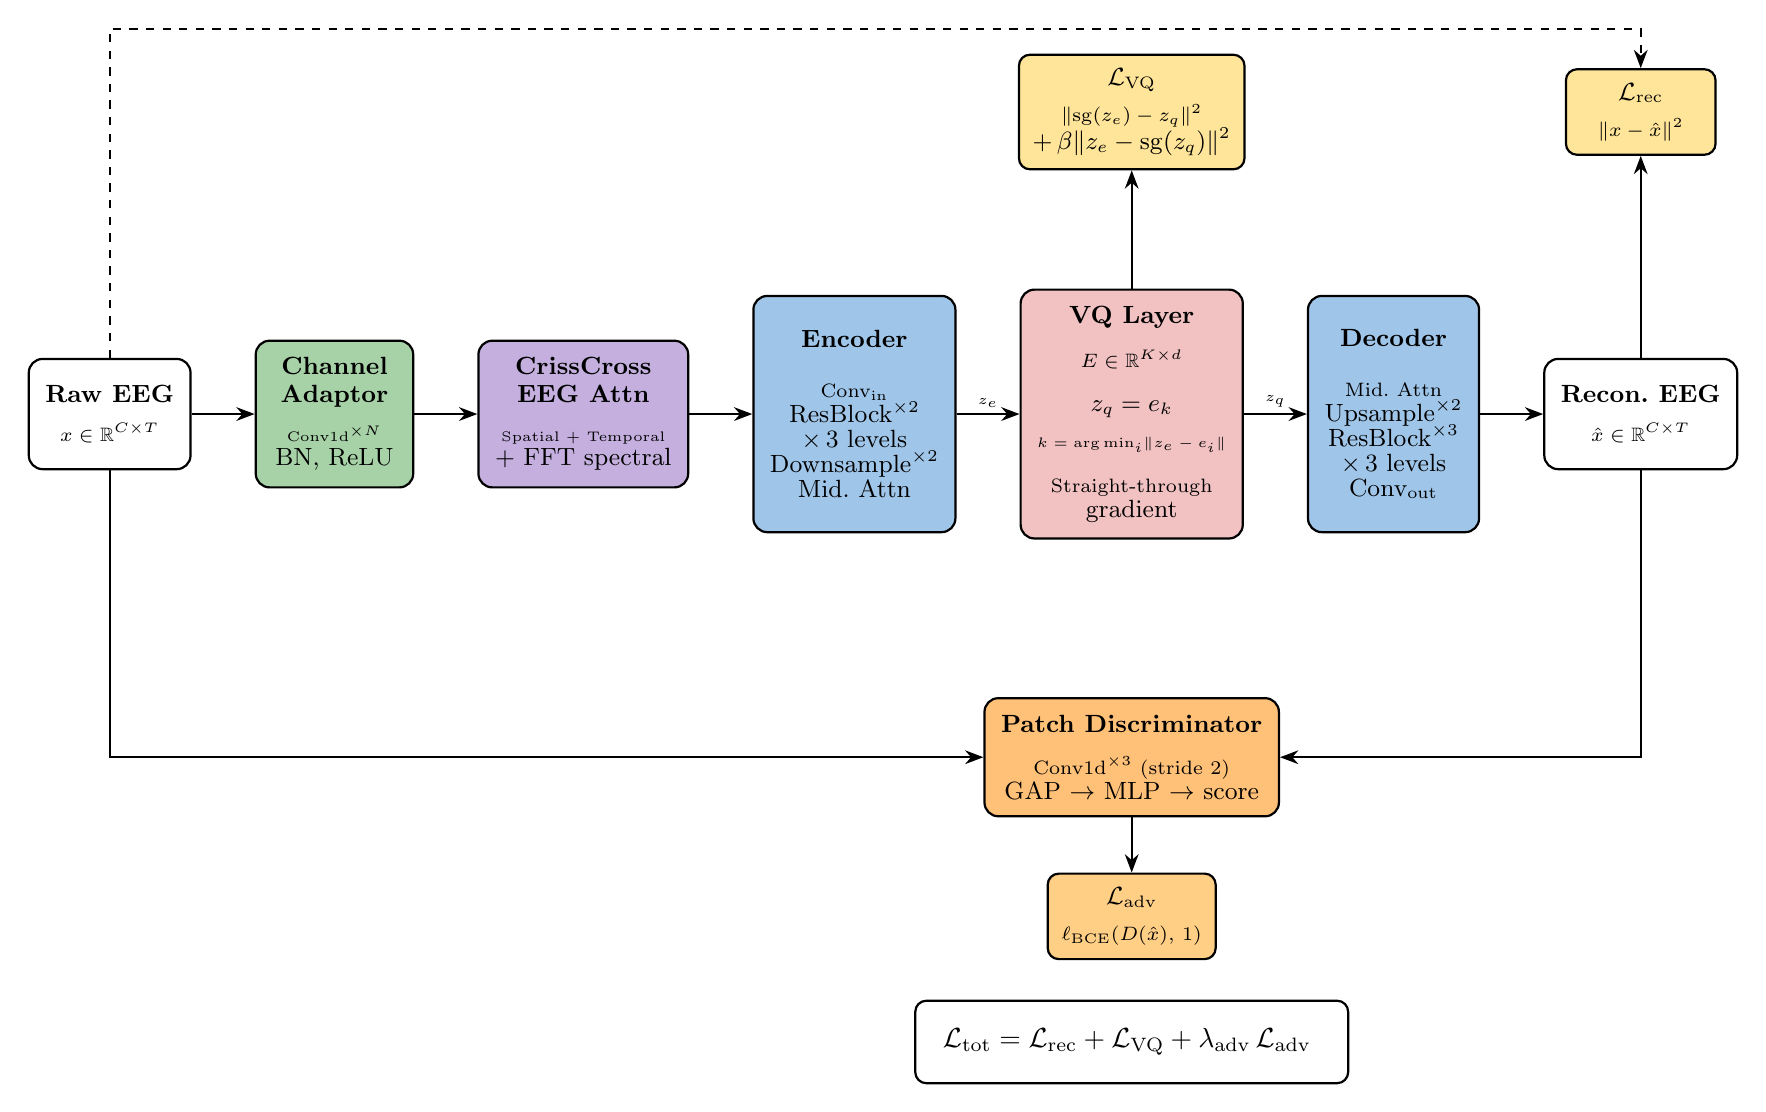
\begin{tikzpicture}[
  >=Stealth, thick,
  block/.style={draw, rounded corners=5pt, align=center, inner sep=6pt,
                font=\small},
  loss/.style={draw, rounded corners=4pt, align=center, fill=cYellow,
               inner sep=5pt, minimum width=1.9cm, font=\small},
  arr/.style={->, thick, >=Stealth}
]

%% ── MAIN PIPELINE ────────────────────────────────────────────────────────────

\node[block, fill=white, minimum width=1.6cm, minimum height=1.4cm] (raw) at (0,0) {
  \textbf{Raw EEG}\\[3pt]
  \scriptsize $x \in \mathbb{R}^{C \times T}$
};

\node[block, fill=cGreen, minimum width=2.0cm, minimum height=1.4cm,
      right=0.8cm of raw] (adapt) {
  \textbf{Channel}\\[-1pt]\textbf{Adaptor}\\[3pt]
  \tiny Conv1d$^{\times N}$\\[-2pt]BN, ReLU
};

\node[block, fill=cPurple, minimum width=2.3cm, minimum height=1.4cm,
      right=0.8cm of adapt] (criss) {
  \textbf{CrissCross}\\[-1pt]\textbf{EEG Attn}\\[3pt]
  \tiny Spatial + Temporal\\[-2pt]+ FFT spectral
};

\node[block, fill=cBlue, minimum width=2.1cm, minimum height=3.0cm,
      right=0.8cm of criss] (enc) {
  \textbf{Encoder}\\[7pt]
  \scriptsize Conv$_{\text{in}}$\\[-2pt]
  ResBlock$^{\times 2}$\\[-2pt]
  ${\times}\,3$ levels\\[-2pt]
  Downsample$^{\times 2}$\\[-2pt]
  Mid.\ Attn
};

\node[block, fill=cRed!60!white, minimum width=2.5cm, minimum height=3.0cm,
      right=0.8cm of enc] (vq) {
  \textbf{VQ Layer}\\[5pt]
  \scriptsize $E \in \mathbb{R}^{K \times d}$\\[5pt]
  $z_q = e_k$\\[2pt]
  \tiny $k = \arg\min_i \lVert z_e - e_i \rVert$\\[5pt]
  \scriptsize Straight-through\\[-2pt]gradient
};

\node[block, fill=cBlue, minimum width=2.1cm, minimum height=3.0cm,
      right=0.8cm of vq] (dec) {
  \textbf{Decoder}\\[7pt]
  \scriptsize Mid.\ Attn\\[-2pt]
  Upsample$^{\times 2}$\\[-2pt]
  ResBlock$^{\times 3}$\\[-2pt]
  ${\times}\,3$ levels\\[-2pt]
  Conv$_{\text{out}}$
};

\node[block, fill=white, minimum width=1.6cm, minimum height=1.4cm,
      right=0.8cm of dec] (recon) {
  \textbf{Recon.\ EEG}\\[3pt]
  \scriptsize $\hat{x} \in \mathbb{R}^{C \times T}$
};

%% ── LOSS BOXES (top) ─────────────────────────────────────────────────────────

\node[loss, above=1.5cm of vq] (l_vq) {
  $\mathcal{L}_{\mathrm{VQ}}$\\[2pt]
  \scriptsize $\lVert\mathrm{sg}(z_e) - z_q\rVert^2$\\[-1pt]
  $+\,\beta\lVert z_e - \mathrm{sg}(z_q)\rVert^2$
};

\node[loss] (l_rec) at (l_vq -| recon) {
  $\mathcal{L}_{\mathrm{rec}}$\\[2pt]
  \scriptsize $\lVert x - \hat{x} \rVert^2$
};

%% ── DISCRIMINATOR (bottom) ───────────────────────────────────────────────────

\node[block, fill=cOrange, minimum width=3.0cm, minimum height=1.5cm,
      below=2.0cm of vq] (disc) {
  \textbf{Patch Discriminator}\\[4pt]
  \scriptsize Conv1d$^{\times 3}$ (stride 2)\\[-2pt]
  GAP $\to$ MLP $\to$ score
};

\node[loss, fill=cOrange!60!cYellow, below=0.7cm of disc] (l_adv) {
  $\mathcal{L}_{\mathrm{adv}}$\\[2pt]
  \scriptsize $\ell_{\mathrm{BCE}}(D(\hat{x}),\,1)$
};

%% ── ARROWS: main data flow ───────────────────────────────────────────────────

\draw[arr] (raw)   -- (adapt);
\draw[arr] (adapt) -- (criss);
\draw[arr] (criss) -- (enc);
\draw[arr] (enc)   -- node[above, font=\tiny, inner sep=2pt] {$z_e$} (vq);
\draw[arr] (vq)    -- node[above, font=\tiny, inner sep=2pt] {$z_q$} (dec);
\draw[arr] (dec)   -- (recon);

%% ── ARROWS: VQ loss ──────────────────────────────────────────────────────────

\draw[arr] (vq.north) -- (l_vq.south);

%% ── ARROWS: reconstruction loss ─────────────────────────────────────────────

\draw[arr] (recon.north) -- (l_rec.south);
\coordinate (routeTop) at ($(l_rec.north) + (0, 0.5cm)$);
\draw[arr, dashed] (raw.north) |- (routeTop) -- (l_rec.north);

%% ── ARROWS: discriminator ────────────────────────────────────────────────────

\draw[arr] (raw.south)   |- (disc.west);
\draw[arr] (recon.south) |- (disc.east);
\draw[arr] (disc.south)  -- (l_adv.north);

%% ── TOTAL LOSS LABEL ─────────────────────────────────────────────────────────

\node[draw, rounded corners=4pt, fill=white, font=\normalsize,
      align=center, inner sep=10pt, below=0.5cm of l_adv] (total) {
  $\mathcal{L}_{\mathrm{tot}} = \mathcal{L}_{\mathrm{rec}}
  + \mathcal{L}_{\mathrm{VQ}}
  + \lambda_{\mathrm{adv}}\,\mathcal{L}_{\mathrm{adv}}$
};

\end{tikzpicture}
\end{document}
